\documentclass{article}

% CoRL 2026 workshop "The UMI Arena", Track 3 (contributed papers): 2-4 pages EXCLUDING acknowledgements
% and references, CoRL main-conference format, single-blind, OpenReview. Topics hit: in-the-wild tracking
% beyond SLAM; the egocentric viewpoint gap between collection and deployment; data scaling/curation.
% Full venue rules and dates: resources/venue.md. Body text lives in sections/*.tex.
\usepackage[preprint]{corl_2026}
\usepackage{graphicx}
\usepackage{booktabs}
\usepackage{xcolor}
\usepackage{siunitx}
\usepackage{multirow}
\newcommand{\todo}[1]{\textcolor{red}{[#1]}}
\newcommand{\grid}[1]{#1}   % numbers from the 2026-10-16 rollout grid (final, 25 scenes; fig/grid_stats.py). Was blue while unfilled.

\title{A Head Camera Is (Almost) All You Need:\\An Electronics-Free UMI Glove Labelled and Observed\\by One Moving Camera}

\author{
  Yosub Shin \\
  University of Hawaii at Manoa \\
  \texttt{yosubs@hawaii.edu} \\
  \And
  Yuan Liu \\
  Independent \\
  \texttt{hiveyuan@gmail.com} \\
  \And
  Igor Molybog \\
  University of Hawaii at Manoa \\
  \texttt{molybog@hawaii.edu} \\
}

\begin{document}
\maketitle

%===============================================================================
\begin{abstract}
A UMI-style device carries a wrist camera for the policy and a pose tracker for the labels: SLAM on that camera, a visual-inertial tracker, a VR controller or a fixed external camera. We replace both with one egocentric camera worn on the collector's head. It sees the fiducial ball and the jaw tags on an otherwise electronics-free glove and the printed tiles taped around the workspace, so every frame carries the gripper's pose in a tile-fixed world frame and the jaw width, with no cable, no IMU and no SLAM. At deployment the same camera rides a cheap servo-driven printed arm beside the robot and keeps the gripper in view the way the head kept the hand in view, driven by a linear viewpoint model fitted on one glove session. The labels are checked against the robot's encoders: \SI{6.5}{mm} median tool-point error, \SI{1.6}{\degree} rotation, \SI{93}{}--\SI{100}{\percent} of frames labelled per session against \SI{78}{}--\SI{92}{\percent} for a fixed external camera that the collector's body hides, and a policy trained on head-camera labels instead of encoders pays \SI{3}{\percent} in validation loss. One person records 2.0--3.1 demonstrations per minute against 1.6 by teleoperation, without occupying the robot, so collectors can work in parallel and a new workspace needs only printed tiles.Adding 194 glove segments to 172 teleoperated episodes lowers ACT's loss on held-out teleoperated episodes from 0.318 to 0.263; added to 48 teleoperated episodes it reaches 0.295, the level of 96--172 teleoperated episodes alone, and on the robot the 48-episode co-trained policy succeeds in \grid{X/25} trials against \grid{X/25} for 48 teleoperated episodes alone and \grid{X/25} for the full 172. Against the conventional wrist-camera recipe and a fixed-camera recipe trained from the same demonstrations the head-camera policy \grid{succeeds in X/25 vs X/25 and X/25}. The glove costs \$22, the camera \$122 and the arm about \$120 in servos and filament; the viewpoint model is naive, so these numbers are a floor for what one moving camera can do. \todo{final numbers from the grid}
\end{abstract}


\begin{figure}[t]
  \centering
  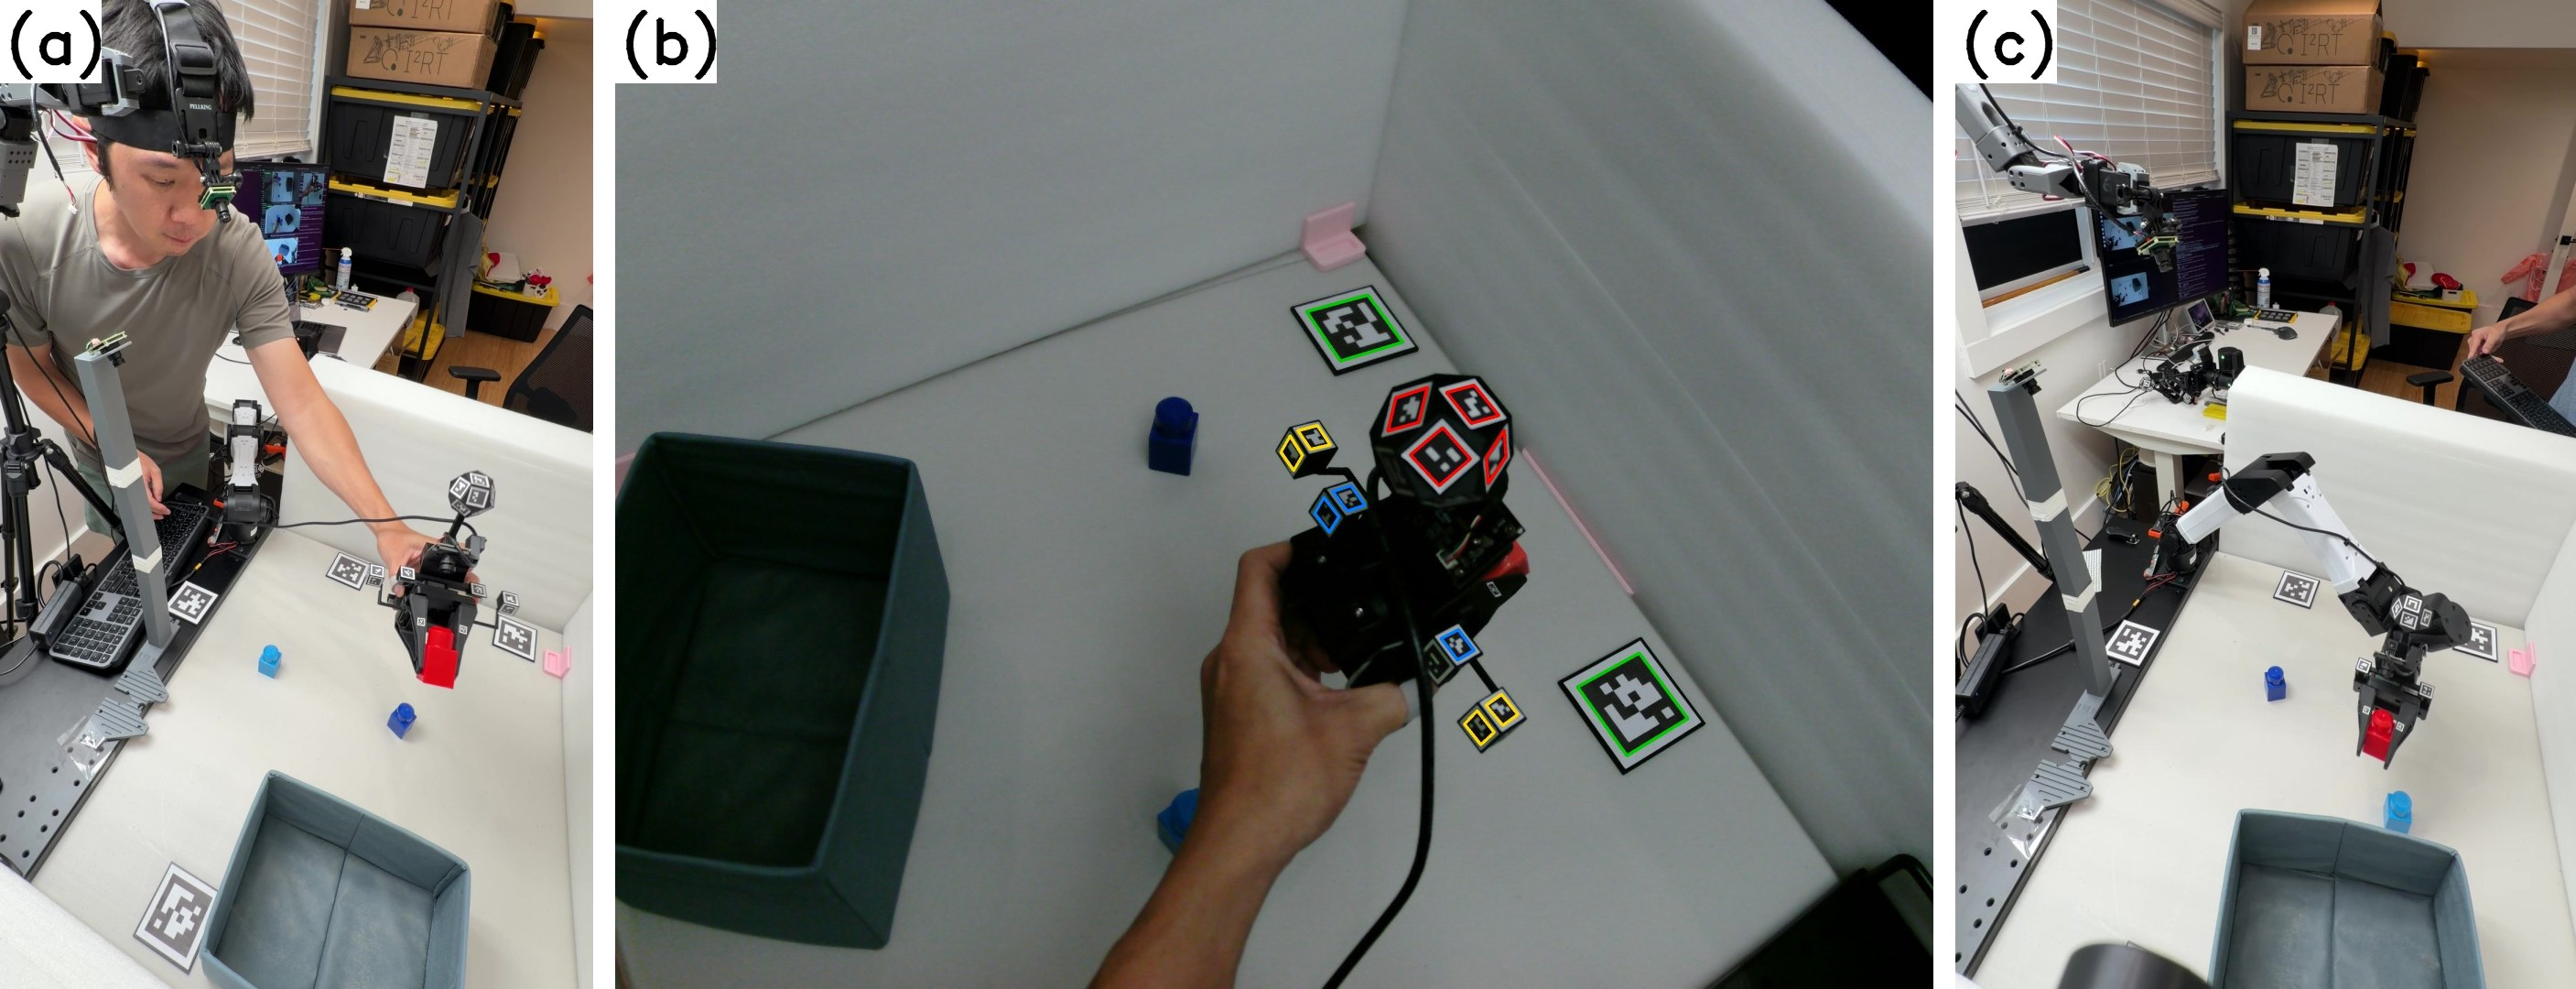
\includegraphics[width=\linewidth]{fig/teaser.jpg}
  \caption{One camera, two mounts. (a) The collector wears the camera on a head strap and carries the electronics-free glove with its fiducial ball over the tiled workspace. (b) The camera's own frame: tiles (green), ball faces (red), jaw tails (blue) and the fixed tags on the gripper back (yellow) give the pose and jaw width. (c) The same camera on the SO-101 positioner beside the YAM during a rollout, same workspace. During collection it is on the collector's head and labels the glove from its own view through the tiles; on the robot the same camera rides a six-joint positioner that follows the gripper. Teleoperated data is recorded through the same positioner, so the three corpora (glove, teleop, rollout) share one viewpoint distribution. Two things in the pictures serve the ablations only: the wrist fisheye and its cable on the glove (a, b) are the observation of the wrist-camera arms, and the fixed camera on the post at the left (a, c) is the observation of the fixed-camera arm and the label source for both; the head-camera system uses neither.}
  \label{fig:teaser}
\end{figure}

%===============================================================================
\section{The idea}
\label{sec:idea}
Teleoperation is limited by robot time: every teleoperated episode occupies the robot as well as the operator. A glove demonstration occupies only the collector. Ours is at least as fast per demonstration as teleoperation of the same task (2.0--3.1 against 1.6 per minute, \S\ref{sec:system}), and none of that time is the robot's: collectors can work in parallel, each one needs a \$22 glove and a \$122 camera, and a new workspace needs only four printed tiles taped around it.

Every UMI-style device answers two questions: what does the policy see, and where was the gripper. The standard answer to the first is a camera on the wrist, which by construction sees what the robot's wrist camera will see. The standard answer to the second is a pose tracker on the same wrist, and every tracker has a price. SLAM over the wrist camera \citep{chi2024umi,campos2021orbslam3} needs a mapping pass for every new scene and enough texture in it, and loses track under occlusion and fast motion; an off-the-shelf visual-inertial tracker adds a second device, a RealSense T265, to the handheld gripper \citep{fastumi2024}; a VR controller in or on the gripper \citep{yubi2026,tinyumi2026} adds weight to the hand (\SI{119}{g} of YUBI's \SI{319}{g}) and brings a tracking system of its own, whose accuracy has to be measured separately \citep{vrtracking2024,quest2rehab2022}; a fixed 4K camera over the workspace, the choice of our earlier glove \citep{yamumi2026}, gives absolute labels but ties collection to the camera's mount, and the collector's own body hides the hand from it, \SI{8}{}--\SI{22}{\percent} of frames per session in the data below (\S\ref{sec:labels}). The wrist camera has prices of its own. It puts electronics on the glove: a camera, a cable and a stream to synchronise with the tracker. And it frames the jaws and little else, so the goal of a carry, here the bin, can leave the policy's view while the task still depends on it: a hand-centric view trades observability of the scene for generalisation \citep{hsu2022hands}.

Two of the open problems this workshop names \citep{umiarena2026} are in-the-wild tracking that does not rest on SLAM, and the viewpoint gap between what a handheld device records and what the robot sees. Our answer to both is one camera, worn. The collector's head tracks the hand by habit, since gaze goes to each object just before the hand acts on it \citep{land2001eye}; it keeps the gripper roughly centred at arm's length and is never occluded by the torso. From its view the fiducial ball gives the pose, the jaw tags give the width, and printed AprilTag \citep{olson2011apriltag} tiles taped on the table give the world frame, so the glove itself carries no electronics at all, and the scene around the gripper, bin included, stays in frame. The same camera is the policy's observation. On the robot a small servo-driven printed arm carries it and imitates the head from the robot's joint state alone, identically during teleoperation and rollouts, so training and deployment share one viewpoint distribution. The price is a moving camera at deployment; the claim is that this price buys the wrist camera, the tracker and the cable, and that the policy is as good. A fixed camera was kept only as an ablation.

Two lines of work are closest. EgoMimic \citep{kareer2025egomimic} co-trains one policy on robot data and egocentric human video from head-worn glasses, with the hand's pose tracked from the video; our collector holds a replica of the robot's gripper, so the contact is the robot's and the jaw width is measured rather than estimated. Active-vision teleoperation \citep{chuang2025avaloha,cheng2024opentelevision} moves a robot camera with the operator's head through a VR headset; our positioner has no operator to follow during rollouts, so it replays a model of how the collector's head moved, from the robot's joint state alone, identically in teleoperation and deployment.


%===============================================================================
\section{System}
\label{sec:system}

\paragraph{Collection.}
The glove is the fiducial-tracked replica of the YAM's gripper \citep{i2rtyam} from \citet{yamumi2026}: the robot's own fingers on a rack-and-pinion linear mechanism, an 11-face \SI{15}{mm} ArUco \citep{garrido2014aruco} dodecahedron on the back of the hand in the manner of DodecaPen \citep{wu2017dodecapen} and, on each jaw, a printed \emph{tail}: a wedge behind the finger carrying \SI{12}{mm} AprilTags on its forward, outer and lower faces, beside a fixed tag on the gripper back. The tails are what makes an electronics-free glove possible. A wrist-camera UMI reads the width from fingertip tags that face its own camera \citep{chi2024umi}; from any camera behind or above the hand those tags are edge-on or hidden (0 of 13.7k frames in our first test), so the width must come from somewhere the head can see. A tail shows at least one face at every hand pose, and its distance to the back tag, projected on the jaw's travel axis in the ball's frame, is the width (\S\ref{sec:labels}). The glove is the \$22 configuration of that device, with the wrist camera and its cable left off: nothing on it is electronic. The collector wears the same Arducam B0587 4K camera and printed mount (\$122) \todo{how it is worn, weight, focus setting} at \SI{15}{Hz}, exposure locked short enough to freeze hand motion. Four \SI{60}{mm} AprilTag tiles are taped around the workspace (Fig.~\ref{fig:teaser}); their relative layout is measured once from the head-camera footage itself (\S\ref{sec:labels}). Two practical rules: the tiles go where the collector's gaze lands during a grasp, so that two are in view from the natural head pose and none under the bin or in the arm's sweep; and no other tag may be in the scene, since the solver trusts every tile id it sees (a spare sheet, or a tag PDF open on a laptop screen, corrupts the world pose). Cameras roll continuously and a key press marks episode boundaries; the collector records 2.0--3.1 pick-and-place demonstrations per minute (median episode \SI{6}{}--\SI{8}{s}), against 1.6 per minute by teleoperation of the same task on the same arm (median \SI{14}{s}).

\paragraph{Labels from the head camera.}
\label{sec:labels}
Each frame yields three things from one image. (i) The camera's pose in the tile frame, from every tile in view; (ii) the ball's pose in the camera, by fused PnP over the visible faces; (iii) the jaw width, from the tails, by a linear map from tail-to-back-tag distance to opening that is calibrated once per unit (on the glove from holds on calipered spacers, \SI{0.9}{}--\SI{3.8}{mm} holdout RMS per tail face; on the robot against its encoders). (i) and (ii) compose to the gripper's pose in the tile frame, and a tile-to-robot-base link, fitted once from a session in which the robot carried the ball (a robot-world calibration \citep{shah2013robotworld} \todo{confirm this is how the link is solved}), maps it into the robot's base frame for the same joint-space IK the teleoperated labels use. Two things make (i) robust on a moving camera. First, the tile layout is refit from the footage: the tile positions declared from the first fixed-camera session were inconsistent at the few-millimetre level, so solves over three or four tiles ran at \SI{3.4}{px} RMS while any pair ran under \SI{1}{px}; refitting the layout from single-tile poses observed in one session brings the four-tile solve to \SI{0.5}{px} and the disagreement between two single-tile camera poses on the same frame from \SI{10}{}--\SI{13}{mm} to \SI{4}{}--\SI{9}{mm} median. Second, frames that show only one tile are chained to the last accepted pose under a motion bound (\SI{0.6}{m/s}, \SI{120}{\degree/s}) instead of being discarded. What remains blind is cut: stretches longer than \SI{0.3}{s} without a label split an episode into segments, and segments under \SI{1}{s} are dropped, so a blind moment costs its frames and not the episode. Per session, \SI{0.7}{}--\SI{7.4}{\percent} of frames are cut this way; the same demonstrations labelled from the fixed external camera lose \SI{8}{}--\SI{22}{\percent}, because the collector's body hides the ball, and fragment into 259 segments where the head camera keeps 200.

\paragraph{The robot's head.}
A six-joint SO-101 follower arm \citep{so101}, printed and driven by six \$14 serial servos (about \$120 in parts\footnote{Follower-only estimate from third-party BOM pages; the official two-arm BOM is about \$230. \todo{confirm on the SO-ARM100 README}}), stands beside the YAM and carries the same camera (Fig.~\ref{fig:teaser}c). The whole addition to a teleoperation rig is therefore under \$250, and the glove is the cheapest part of it. At the start of a session it parks at the median head pose of the glove sessions, closed-loop against the tiles, and calibrates its own view axes against them. During teleoperation and during rollouts it reads only the YAM's joint state: forward kinematics gives the gripper's position, a fixed gain keeps the gripper's bearing in the camera where it was at park, and a residual model fitted on the glove sessions reproduces how the head's viewpoint depends on the hand's position. Commands pass through a low-pass filter, a rate cap of \SI{50}{\degree/s} and a workspace box, and the resulting camera motion lags the gripper by about \SI{0.4}{s}, with a median camera position error of \SI{16}{mm} (\SI{34}{mm} p90) against the tiles. The gripper's framing in the robot's head-camera footage (centroid at 0.37/0.62 of the image width/height) matches the collector's (0.38/0.60). The kinematic model of the arm is fitted once from 60 tile-verified poses (\SI{7}{mm}/\SI{0.7}{\degree} residual) and the camera is released to the recorder after calibration; the positioner is otherwise invisible to the policy.

\paragraph{Datasets.}
Teleoperation under the positioner gave 178 episodes (38.6k frames at \SI{15}{Hz}); 6 are held out as the validation set for every arm. Four glove sessions gave 198 demonstrations, 200 segments after blind cutting (50.0k frames), 6 held out. Every policy is ACT \citep{zhao2023act} trained with LeRobot \citep{lerobot2024}: one recipe, 50k steps, joint-space actions, best checkpoint by validation loss on the robot's held-out episodes. The glove timeline is resampled to teleoperation pace and the measured width is mapped to the robot's commanded value, as in \citet{yamumi2026}, with one change that mattered: the closed-on-object anchor of that map is the squeeze level teleoperators actually command (the per-episode minimum, 0.22 of the stroke), not their median grasp command (0.25). With the median anchor an earlier version of every glove policy opened during the carry; with the squeeze anchor none of the head-view policies below drops the block.


%===============================================================================
\section{Experiments}
\label{sec:results}

\paragraph{Design.}
In every arm the teleoperated half carries the robot's encoder labels; only the glove half carries the camera under test, and its observation is whichever camera the arm deploys. Table~\ref{tab:arms} lists the eight arms. Arms 1--4 are the device and its budget pair; arm 6 checks the labels; arms 5, 7 and 8 compare cameras, arm 5 being the conventional wrist-camera recipe \citep{chi2024umi}. All glove arms train on the same 198 demonstrations. Arms 5 and 8 observe through a wrist fisheye that was mounted on the glove for this ablation only; the head-view arms use the glove with no electronics. The fixed-camera arms train on \SI{10}{\percent} fewer glove frames (43.5k against 48.5k), which is the occlusion cost of the fixed camera and not a budget choice.

\begin{table}[t]
  \centering
  \footnotesize
  \caption{The eight policies. Teleop labels are encoders except arm 6. Robot val = ACT loss on the 6 held-out teleoperated episodes (encoder targets, comparable across all rows; arm 6 is scored on the encoder targets too). Rollouts: \grid{25} placements, one trial each, \SI{60}{s} budget; failure modes n = no grasp, d = dropped before the bin, b = dropped at the bin. \todo{fill from the grid}}
  \label{tab:arms}
  \setlength{\tabcolsep}{4pt}
  \begin{tabular}{clllcccl}
    \toprule
    \# & arm & glove labels & observation & teleop + glove & val & success & fails \\
    \midrule
    1 & teleop only & --- & head cam & 172 & 0.318 & \grid{/25} & \grid{} \\
    2 & \textbf{device} & head cam & head cam & 172 + 194 & \textbf{0.263} & \grid{/25} & \grid{} \\
    3 & teleop only, low budget & --- & head cam & 48 & 0.464 & \grid{/25} & \grid{} \\
    4 & device, low budget & head cam & head cam & 48 + 194 & 0.295 & \grid{/25} & \grid{} \\
    5 & wrist-camera UMI & fixed cam & wrist fisheye & 168 + 253 & 0.257 & \grid{/25} & \grid{} \\
    6 & head-cam teleop labels & --- & head cam & 172 (head labels) & 0.328 & \grid{/25} & \grid{} \\
    7 & fixed camera as system & fixed cam & fixed cam & 172 + 255 & 0.256 & \grid{/25} & \grid{} \\
    8 & head labels, wrist view & head cam & wrist fisheye & 168 + 192 & 0.252 & \grid{/25} & \grid{} \\
    \bottomrule
  \end{tabular}
\end{table}

\paragraph{Label accuracy.}
With the ball on the YAM and the encoders as reference, the head-camera chain places the tool point with \SI{6.5}{mm} median / \SI{14.1}{mm} p90 error and \SI{1.55}{\degree} / \SI{2.70}{\degree} rotation (5\,065 frames, \SI{91}{\percent} inliers), after the one-time base link absorbs the constant offset. The jaw width is checked the same way: on 112 teleoperated episodes (24.6k frames) the head-camera width is within \SI{3.5}{\percent} of the stroke of the encoder value at the median (\SI{7.9}{\percent} p90; about 3 and \SI{7.5}{mm} of the \SI{95}{mm} stroke), \SI{2.3}{\percent} in the closed state that decides a grasp, with no lag (a one-frame shift raises the error) and a label on every frame in 9 of 10 episodes (worst \SI{68}{\percent}). The residual is a systematic under-read of \SI{4}{}--\SI{6}{\percent} at full opening, a scale error of the per-session fit rather than noise. \todo{Yuan: a check on unseen openings across viewing angles, with coverage per angle, would make this a proper instrument table.} Downstream, a policy trained on head-camera labels instead of encoders (arm 6 against arm 1), scored on the same encoder-labelled held-out episodes, reaches 0.328 against 0.318, a \SI{3}{\percent} price for the labels, and succeeds in \grid{X/25} rollouts against \grid{X/25}.

\paragraph{Co-training and the teleoperation budget.}
Glove and teleoperated episodes are co-trained as one merged dataset, as robot data from different sources has been before \citep{fu2024mobilealoha,kareer2025egomimic}. Adding the glove set to all 172 teleoperated episodes lowers the robot-validation loss from 0.318 to 0.263 (\SI{17}{\percent}); added to 48 teleoperated episodes it lowers it from 0.464 to 0.295. Fig.~\ref{fig:budget} shows the full curve: the glove set is worth 65--100 teleoperated episodes by log-linear interpolation of the teleop-only curve, i.e. 2--3 glove demonstrations per teleoperated one, and the 48-episode mix lands between 96 and 172 teleoperated episodes alone. In robot time, the glove set saves about 50--120 teleoperated episodes at the 48-episode budget.The gain shrinks with budget (0.075 at 24 episodes down to 0.011 at 96, measured against the full mix), so glove data stretches a small teleoperated set but does not replace the last few dozen episodes. On the robot \grid{the 48-episode mix succeeds in X/25 against X/25 for the 48 teleoperated episodes alone and X/25 for the full 172}, \todo{with the recovery behaviour of the mix: in scene 5 the mix missed its first grasp, backed off and re-grasped, where the teleop-only policy never closed in}.

\begin{figure}[t]
  \centering
  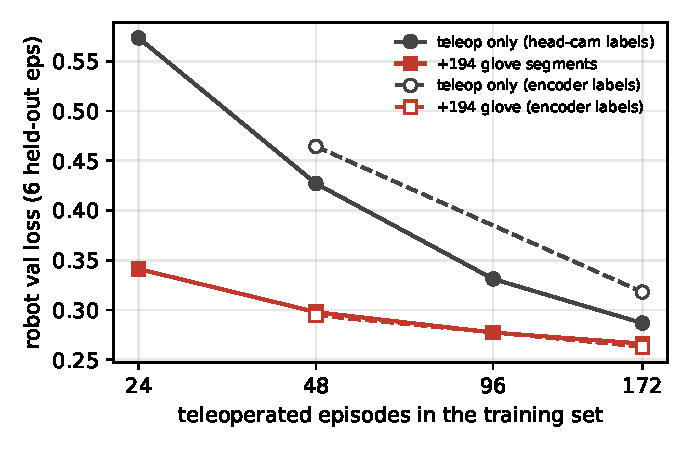
\includegraphics[width=0.6\linewidth]{fig/budget.pdf}
  \caption{Robot validation loss against the number of teleoperated episodes, with and without the 194 glove segments. Solid: head-camera-labelled teleoperation (round-2 chain, four budgets); dashed: encoder-labelled teleoperation (final design, two budgets). The glove set moves every budget to the level of 2--4$\times$ as many teleoperated episodes.}
  \label{fig:budget}
\end{figure}

\paragraph{Which camera.}
Offline, the four co-trained arms with different cameras (2, 5, 7, 8) sit within 0.011 of each other, and each gains 0.04--0.06 over its teleop-only twin, so the validation loss does not separate the cameras; offline loss is known to be a weak proxy for rollout success \citep{mandlekar2021robomimic}. The rollouts do. \grid{Arm 2 succeeds in X/25, the wrist-camera recipe in X/25, the fixed camera in X/25, and head labels on the wrist view in X/25.} The failure modes split by camera: head-view policies fail by never grasping, wrist-view policies by dropping the block during the carry, \grid{d+b = X of Y failures for arms 5 and 8 against X of Y for arms 1--4}. \todo{every observed wrist-view drop happened while the bin was outside the fisheye's view; no drop was observed with the bin in view; the head camera keeps gripper and bin in frame throughout the carry.} Holding the labels fixed (arm 8 against arm 2) isolates the observation; holding the observation fixed (arm 8 against arm 5) isolates the label source: \grid{result}. The fixed camera (arm 7) \grid{result}; note that it was mounted low because the positioner occupied the elevated vantage point, so its occlusion rate is an upper bound for a fixed camera in this workspace.

\begin{figure}[t]
  \centering
  \fbox{\parbox[c][4.2cm][c]{0.96\linewidth}{\centering \todo{Rollout protocol figure as in the device paper: the 25 placements with per-scene success over the 8 arms; ghost-alignment inset. Generate from rollout\_logs/grid\_20261016 (placements.json, scene*\_ref.png, trials.jsonl).}}}
  \caption{Rollout protocol. \grid{25} placements, each scene's block re-placed to a saved reference for every arm (ghost alignment), arm order shuffled per scene, \SI{60}{s} budget.}
  \label{fig:placements}
\end{figure}

\paragraph{Anecdotes.}
\todo{Transcribe from rollout\_logs/grid\_20261016/anecdotes.md: scene-5 budget pair; mix\_gHA opening mid-carry with the block out of view; wrist drops only when the bin is out of view.}


%===============================================================================
\section{Limitations and what is next}
\label{sec:discussion}
The tile layout is refit from one session by median single-tile poses rather than bundle-adjusted; a proper adjustment should bring the single-tile jitter below the current \SI{4}{}--\SI{9}{mm}. The positioner lags the gripper by \SI{0.4}{s} and hits joint limits on the largest sweeps; a lighter camera or a faster arm would close that. The head camera also sees the collector's arm and the glove's fingers, which is the appearance gap that keeps glove-only policies from transferring (robot-validation loss 0.52 against 0.26 co-trained), as in the fixed-camera version of the device. The fixed-camera ablation was mounted low because the positioner took the high vantage point; a higher fixed camera would occlude less, though it cannot follow the hand. Hardware and software are open \citep{yamumi2026,forwardcamumi2026}. \todo{what is next: multi-tile workspaces, in-the-wild sessions, a second task}


%===============================================================================
\bibliography{refs}

\end{document}
